% Giacomo Petrillo
% lezione di Punzi

\subsection{Costruzione di Neyman}

Ora passiamo alla stima intervallare vera e propria.
Se non abbiamo un priore e quindi neanche un posteriore,
non possiamo calcolare la probabilità di una regione nello spazio del parametro.
Tuttavia una stima intervallare è una statistica,
quindi è definito il concetto di probabilità che la regione contenga il valore vero.
Quindi, anziché richiedere che la regione abbia probabilità almeno $\mathrm{CL}$,
chiederemo che,
qualunque sia il valore vero,
la probabilità che la regione contenga il valore vero è almeno $\mathrm{CL}$.

\begin{definition}[Coverage]
	Con la notazione della \autoref{th:cred},
	il \emph{coverage} di $f$ calcolato in $\theta$ è
	\begin{equation*}
		\cvg_f(\theta)
		\is \int_{f(x)\ni\theta} \de x\, p(x;\theta);
	\end{equation*}
	il livello di confidenza\footnote{Purtroppo viene chiamato nello stesso modo che nel caso bayesiano.} è
	\begin{equation*}
		\mathrm{CL}
		= \inf_\theta \cvg_f(\theta).
	\end{equation*}
\end{definition}

Osserviamo che,
se cambiamo parametro,
i coverage e quindi il livello di confidenza non cambiano.

\begin{figure}
	\centering
	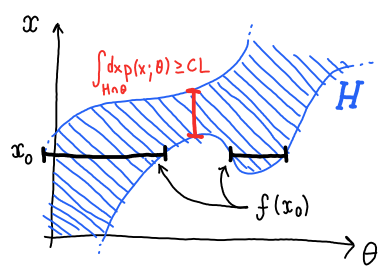
\includegraphics[width=18em]{banda}
	\caption{\label{fig:neyman}%
	Costruzione di Neyman: banda di confidenza.}
\end{figure}

Il problema ora è costruire $f$ in modo da avere un certo $\mathrm{CL}$.
Esponiamo la \emph{costruzione di Neyman} (vedi \autoref{fig:neyman}).
Consideriamo una \emph{banda di confidenza} $H\subseteq \Theta\times X$,
tale che le probabilità delle sezioni a parametro fisso siano almeno $\mathrm{CL}$:
\begin{equation}
	\label{eq:neycov}
	\forall\theta:
	\int_{H\cap \{\theta\}} \de x\, p(x;\theta) \ge \mathrm{CL}.
\end{equation}
Se definiamo la stima intervallare come le sezioni di $H$ a variabile costante
\begin{equation*}
	f(x) \is H \cap \{x\}
\end{equation*}
otteniamo che
\begin{align*}
	f(x)\ni\theta
	\iff
	H \cap \{x\} \ni \theta
	\iff
	(\theta,x) \in H
	\iff
	x \in H \cap \{\theta\}
\end{align*}
e quindi l'integrale della \eqref{eq:neycov} è proprio il coverage.
Adesso il problema si è spostato a scegliere $H$
cioè a scegliere per ogni $\theta$ una regione di $x$ che abbia probabilità almeno $\mathrm{CL}$.
Come nel caso bayesiano, possiamo usare una funzione di ordinamento.
Il modo più intuitivo di scegliere la funzione di ordinamento è il \emph{probability ordering} cioè
\begin{equation*}
	O(\theta,x) = p(x;\theta),
\end{equation*}
tuttavia se cambiamo variabile la regione definita con il probability ordering trasforma in modo non banale,
quindi non è in qualche modo intrinseca.

\begin{example}
	\label{th:poisssup}
	Consideriamo la poissoniana.
	Supponiamo di voler mettere un ``limite superiore'' a $\mu$,
	cioè di voler calcolare una stima intervallare che dia come risultato un intervallo che parte da~0.
	Allora la banda di confidenza deve essere delimitata inferiormente da una curva crescente,
	quindi scegliamo la funzione di ordinamento $O(\mu,k)=k$.
	Limitiamoci al caso $k=0$.
	Vogliamo che
	\begin{equation*}
		\sum_{k=k_\mathrm{min}}^\infty \frac{\mu^k}{k!}e^{-\mu} \ge \mathrm{CL},
	\end{equation*}
	quindi per i $\mu$ tali che il termine $k=0$ della somma è maggiore di $1-\mathrm{CL}$,
	$\mu$ è nella stima intervallare.
	Quindi
	\begin{align*}
		e^{-\mu_\mathrm{max}}
		&= 1 - \mathrm{CL} \implies \\
		\implies \mu_\mathrm{\max}
		&= -\log(1-\mathrm{CL}).
	\end{align*}
	Notiamo che abbiamo ottenuto lo stesso risultato dell'esempio bayesiano\footnote{Vedi \autoref{th:poissbayes}.} con priore uniforme,
	e che tuttavia questa è una futile coincidenza!
\end{example}

\begin{example}
	\label{th:unifunosup}
	Consideriamo la distribuzione uniforme.
	Usiamo la funzione di ordinamento $O(m,x)=x$.
	\begin{align*}
		x_\mathrm{max}
		&= m, \\
		\mathrm{CL}
		&= \int_{x_\mathrm{min}}^m \frac{\de x}{m} = \\
		&= 1 - \frac m{x_\mathrm{min}} \implies \\
		\implies m_\mathrm{min}
		&= x, \\
		m_\mathrm{max}
		&= \frac x{1-\mathrm{CL}}.
	\end{align*}
\end{example}

\begin{exercise}
	\label{th:unifsup}
	Estendere l'\autoref{th:unifunosup} al caso di $N$ estrazioni.
\end{exercise}

\begin{solution}
	Usare il fatto che $\max \mathbf x$ è una statistica sufficiente.
	\marginpar{Spiegare in che modo basta usare una statistica sufficiente.}
	Risulta
	\begin{align*}
		m_\mathrm{min}
		&= \max\mathbf x, \\
		m_\mathrm{max}
		&= \frac{\max\mathbf x}{\sqrt[N]{1-\mathrm{CL}}}.
	\end{align*}
\end{solution}

\paragraph{Relazione tra coverage e credibilità}

In ambito bayesiano, calcoliamo il valore atteso della credibilità:
\begin{align*}
	E_x[\cred_f(x)]
	&= \int \de x\, p(x)
	\int_{f(x)} \de\theta\, p(\theta|x) = \\
	&= \int \de x\, \int_{f(x)} \de\theta\,
	p(x) \frac{p(x|\theta) p(\theta)}{p(x)} = \\
	&= \int \de \theta\, p(\theta)
	\int_{f(x)\ni\theta} \de x\, p(x|\theta) = \\
	&= \int \de \theta\, p(\theta) \cvg_f(\theta) = \\
	&= E_\theta[\cvg_f(\theta)].
\end{align*}
A causa di questa proprietà la gente si confonde e pensa che ci siano relazioni mistiche tra gli intervalli estratti da posteriori bayesiani e le stime intervallari,
ma questo conto non ha senso in ambito frequentista perché ci sono $p(\theta)$ e $p(x)$.
